% =====================================================================================
% hetlearn: heterogeneous expectations, adaptive learning and switching in IRIS models
% Manuscript for Computational Economics (Springer), Springer Nature LaTeX template
% (sn-jnl.cls, version 3.1, December 2024), reference style sn-basic (author-year).
%
% Overleaf: upload the contents of this folder, Menu > Compiler: pdfLaTeX, main document
% main.tex. Needs sn-jnl.cls and sn-basic.bst in the root (both included), figures/*.pdf and
% tables/*.tex. Locally: pdflatex main; bibtex main; pdflatex main; pdflatex main.
% The three \input lines pull in tables/*.tex, unchanged copies of paper/tables/ written by
% paper/figures/make_figures.py. Each is wrapped as {\let\small\relax\setlength{\tabcolsep}{4pt}...}
% so it keeps the class table font (8bp) and fits the 31pc text width. sn-jnl wraps every
% table in threeparttable, so a tabular must not be put inside \resizebox or adjustbox.
% Springer asks for a single .tex file at submission: paste the three files in place of their
% \input lines then.
% Written 2026-10-22 without a LaTeX installation: braces, environments, labels, references
% and citation keys were checked with a script, but the file has not been compiled yet.
% =====================================================================================

\documentclass[pdflatex,sn-basic]{sn-jnl}

\usepackage{graphicx}
\usepackage{amsmath,amssymb,amsfonts}
\usepackage[title]{appendix}
\usepackage{xcolor}
\usepackage{textcomp}
\usepackage{booktabs}
\usepackage{array}
\usepackage{listings}

% Inline code: option names, file names, MATLAB identifiers. \detokenize prints underscores,
% braces and quotes literally; do not put %, # or a backslash inside \code{...}.
\DeclareRobustCommand{\code}[1]{\texttt{\detokenize{#1}}}

\lstdefinestyle{cfg}{language=Matlab,
  basicstyle=\ttfamily\fontsize{8}{9.5}\selectfont,
  columns=fullflexible,
  keepspaces=true,
  upquote=true,
  showstringspaces=false,
  breaklines=true,
  frame=single,
  framerule=0.2pt,
  rulecolor=\color{black!35},
  backgroundcolor=\color{black!3},
  commentstyle=\color{black!60}\itshape,
  keywordstyle=\bfseries,
  aboveskip=6pt,
  belowskip=6pt}
\lstset{style=cfg}

% Notation (as in the technical appendix of the repository)
\newcommand{\RE}{\mathrm{RE}}
\newcommand{\BR}{\mathrm{BR}}
\newcommand{\fRE}{f^{\RE}}
\newcommand{\fBR}{f^{\BR}}
\newcommand{\Eagg}{\tilde{E}}
\newcommand{\FE}{\mathit{FE}}
\newcommand{\transp}{^{\prime}}

\emergencystretch=1.5em
\raggedbottom

\begin{document}

\title[hetlearn: heterogeneous expectations in IRIS models]{hetlearn: a toolbox for heterogeneous expectations, adaptive learning and switching in IRIS models}

\author*[1]{\fnm{Tolga} \sur{\"Ozden}}\email{[email to be added]}

% TODO(author): affiliation.
\affil*[1]{\orgname{[Affiliation to be added]}}

\abstract{Models with adaptive learning and heterogeneous expectations are usually solved with
code written for one paper, one model and one set of timing assumptions. This paper presents
hetlearn, a MATLAB toolbox that adds heterogeneous expectations to any IRIS model with
forward-looking terms. The user supplies a model file, parameters and data. The toolbox rewrites
the model so that chosen one-step expectations are a population mix of rational agents and
adaptive learners, learns beliefs and population shares over the history, and forecasts one
quarter at a time while beliefs and shares are updated. Options cover the information sets of
both agent types, anchored or model-consistent rational agents, perceived laws of motion from an
AR(1) to a VAR(1), initial beliefs, constant and endogenous gains, discrete-choice switching, a
projection facility, and three ways of building the history: learning on the
rational-expectations filter, inverting the learning model, or a time-varying Kalman filter.
Conditional forecasts with backed-out shocks, Ramsey policy, density forecasts, shock
decompositions and real-time forecast evaluation build on the forecast stage, and seven further
expectation rules from the bounded-rationality literature are included. The toolbox has been
tested on linear models. In an illustration with the Smets--Wouters model, forecasting from the
2022 US inflation peak, average inflation over the following four years is 3.45\% with learners
on inflation against 2.59\% under rational expectations. The paper describes the tools; it does
not answer a research question.}

\keywords{adaptive learning, heterogeneous expectations, DSGE models, scenario analysis, IRIS toolbox, MATLAB}

\pacs[JEL Classification]{C63, D84, E37, E52}

\maketitle

% =====================================================================================
\section{Introduction}\label{sec:intro}
% =====================================================================================

Most DSGE and semi-structural models used for forecasting and policy analysis assume rational
expectations (RE). A long literature replaces that assumption with adaptive learning, in which
agents forecast with a simple perceived law of motion (PLM) and re-estimate it as data arrive
\citep{sargent1999,evans2001,evans2009}, or with heterogeneous expectations, in which agents
choose among forecasting rules according to their past performance
\citep{brock1997,branch2009,branch2010,hommes2011,hommes2021}. Estimated versions of these
models exist for small New Keynesian models and for the medium-scale model of \citet{smets2007}
\citep{milani2007,slobodyan2012a,slobodyan2012b,cornea2019,hmoz2023,ozden2025}, and the
mechanism has been used to study credibility, wage-price spirals and the anchoring of inflation
expectations \citep{hommes2019,carvalho2023,koz2024}.

Each of these studies comes with its own code, written for one model and one set of
assumptions: the PLM, whether learners see current data, whether the rational agents know that
others learn, how initial beliefs are set, whether the gain is constant, and what happens when
beliefs become explosive. These choices matter for the results, and papers make them
differently. They are rarely varied within one study, because in hand-written code each of them
is costly to change. For a modeler at a central bank who wants to know how a projection changes
when part of the public learns, the entry cost is high: the expectation block has to be derived
and coded for the institution's own model, and then kept consistent with every later change to
that model.

This paper presents \code{hetlearn}, a MATLAB toolbox built on the IRIS toolbox \citep{iris} to
lower that cost. IRIS is a MATLAB package for DSGE and semi-structural models that parses a model
file, solves it under RE, runs the Kalman filter and simulates it; it is a common tool for
projection models of the kind described by \citet{berg2006}. The
toolbox is plug and play for any IRIS model with forward-looking terms. The user brings a model
file, a parameter file and a database. The toolbox finds every lead of a transition variable,
writes an extended model in which the one-step expectations of the chosen variables are a
population mix of RE agents and adaptive learners, and checks that the extended model collapses
to the original one when every agent is rational. It then learns beliefs and population shares
over the history and forecasts one quarter at a time, re-solving the model whenever beliefs or
shares change. A scenario is a short MATLAB function; the same scenario runs under RE or under
learning by changing one option, and a child scenario inherits everything from its parent and
sets only what differs.

The toolbox is meant as a common framework for the analyses in this literature. It contains the
learning and switching block of \citet{ozden2025}, in which anchored RE agents and AR(1)
learners switch on past forecast errors; the endogenous gain of \citet{koz2024}; the RE and
adaptive predictors of \citet{branch2009,branch2010}; PLMs in the spirit of the small
forecasting models of \citet{slobodyan2012a} (AR(1), AR(2) and VAR(1), without their
Kalman-filter learning);
learning on every forward-looking variable as in \citet{milani2007}; and the recursive least
squares and projection facility of \citet{evans2001}. Section~\ref{sec:lit} maps these studies
to the options.

The intended users are modelers in central banks and other institutions, and researchers who run
scenario analysis with DSGE or semi-structural models: anyone who wants to put a learning or
switching assumption next to the RE projection of an existing model. The paper is a proof of
concept. It motivates the toolbox, describes the tools and how they can be extended, and
illustrates them; it does not answer a research question, and it does not describe the
properties of any model. The toolbox has been tested on linear models with linear solutions
only. Nothing in its design rules out a nonlinear IRIS model, and a code path exists for one,
but no test covers it. The toolbox takes model parameters as given and does not estimate them.

The illustrations use the model of \citet{smets2007} (SW07) with its published parameters on US
data from 1966 to 2026, and forecast from the inflation peak of 2022Q2. With inflation
expectations split between anchored RE agents and AR(1) learners, average inflation over
2022Q3--2026Q2 is 3.45\% in the learning economy against 2.59\% under RE, mainly because the
learners enter the forecast with a perceived AR(1) coefficient of 1.06 after the 2021--22 surge. The same
scenario is then run with a policy deviation from the Taylor rule, under Ramsey policy, as a
density forecast and with alternative PLMs. The other tools are described and are available in
the repository.

The documentation website, \url{https://tolgaozden.github.io/iris_toolbox_learning/},
% TODO(author): the site is built but not yet deployed (GitHub Pages must be switched on).
covers installation, a tutorial for the first application, every option with an example and a
guide for adding a model. The technical appendix in the repository
(\code{docs/technical_appendix/}) gives the mathematics, assumptions and defaults of every option
of the core toolbox and is the reference for the details this paper leaves out; the further
expectation rules of Section~\ref{sec:rules} are documented in the user guide and on the website.

Section~\ref{sec:lit} places the toolbox in the literature and among existing software.
Section~\ref{sec:design} describes how a run works. Section~\ref{sec:options} presents the
options. Section~\ref{sec:sw07} gives the SW07 illustrations. Section~\ref{sec:rules} describes
seven further expectation rules. Section~\ref{sec:extend} explains how the toolbox can be
extended and lists its limitations, and Section~\ref{sec:concl} concludes.

% =====================================================================================
\section{Expectation formation in the literature and in the toolbox}\label{sec:lit}
% =====================================================================================

\subsection{What the toolbox nests}\label{sec:nests}

Adaptive learning in macroeconomics starts from the idea that agents behave like econometricians:
they forecast with a reduced-form model and update its coefficients by recursive least squares
(RLS) as new data come in \citep{marcet1989,evans2001}. With a decreasing gain, beliefs can
converge to the RE equilibrium; with a constant gain, agents keep discounting old data and
beliefs keep moving, which is the version used in most estimated models. \citet{milani2007} estimated
a New Keynesian model in which every forward-looking expectation is learned with a constant gain
and found that learning can replace part of the mechanical persistence (habits, indexation) that
RE models need. \citet{slobodyan2012a,slobodyan2012b} did the same for SW07, with PLMs ranging
from small forecasting models to the full minimum-state-variable form, and found that the
specification of the PLM shapes both fit and dynamics. \citet{eusepi2011} and \citet{milani2011}
used learning to generate expectation-driven fluctuations.

Heterogeneous expectations add a population of forecasting rules. In \citet{brock1997} agents
choose among predictors with a logit in their past performance; \citet{branch2004} found that
this describes survey data on inflation expectations. \citet{branch2009,branch2010} put RE and
adaptive predictors in a New Keynesian model, first with fixed and then with switching shares;
\citet{massaro2013} derived the aggregate equations from individual decisions;
\citet{degrauwe2011}, \citet{anufriev2012} and \citet{hommes2013,hommes2021} studied heuristic
switching more broadly, and \citet{cornea2019} estimated it on US inflation.
\citet{hommes2019} read the share of agents who believe the inflation target as central-bank
credibility. \citet{ozden2025} combines both strands in an estimated model: RE agents, whose
forecast is anchored at the pure-RE solution, and AR(1) learners, whose shares switch on past
squared forecast errors. \citet{koz2024} add an endogenous gain that rises when forecast errors
keep their sign. \citet{hommeszhu2014} and \citet{hmoz2023} study AR(1) forecasting rules whose
coefficients are consistent with the moments of the data they generate.

Table~\ref{tab:nests} lists, for the main reference points, the hetlearn options that come
closest to each setup, and what is not covered. The mapping is about the expectation side only:
the toolbox does not estimate parameters, and a study's results depend on its own model and
estimates. It shows that the same machinery spans the range from every agent rational to every
agent learning, with fixed or switching shares in between.

\begin{table}[tbp]
\centering
\setlength{\tabcolsep}{4pt}
\caption{Published setups and the nearest hetlearn configuration}
\label{tab:nests}
\begin{tabular}{>{\raggedright\arraybackslash}p{2.8cm}>{\raggedright\arraybackslash}p{4.0cm}>{\raggedright\arraybackslash}p{5.1cm}}
\toprule
Study & Expectation side & Nearest hetlearn setting; not covered \\
\midrule
\citet{evans2001} & RLS learning of a PLM; projection facility & \code{beliefs.update = 'rls'}; \code{projection.facility}. Decreasing gain: not included \\
\addlinespace
\citet{milani2007} & every forward-looking variable learned, constant gain & \code{expectations.mode = 'learning'}, \code{variables = 'all'}, \code{gain.rule = 'constant'}; PLM by \code{beliefs.plm.by_var} or a VAR \\
\addlinespace
\citet{slobodyan2012a,slobodyan2012b} & learning in SW07 with small forecasting models or larger PLMs & AR(1), AR(2), regression and VAR(1) PLMs per forward-looking variable. Kalman-filter learning: not included \\
\addlinespace
\citet{branch2009,branch2010} & RE and adaptive predictors with lagged information; fixed or switching shares & \code{'ar1_noconst'} PLM with \code{beliefs.update = 'fixed'}; \code{'fixed_shares'} or \code{'switching'}; \code{beliefs.info = 'lagged'}. Cost of the RE predictor: not included \\
\addlinespace
\citet{brock1997}; \citet{hommes2019} & logit switching between predictors; target believers & discrete-choice switching with memory; a fixed-rule agent type forecasting the steady state (Section~\ref{sec:rules}) \\
\addlinespace
\citet{ozden2025} & anchored RE agents and AR(1) learners, constant gain, period-$t$ information, one share driven by inflation and output-gap errors & \code{re_variant = 'anchored'}, \code{beliefs.info = 'current'}, \code{shares.structure = 'universal'} with two master variables \\
\addlinespace
\citet{koz2024} & endogenous gain (adaptive step size) & \code{gain.rule = 'koz'} \\
\addlinespace
\citet{gaspar2006}; \citet{molnar2014} & optimal policy when the private sector learns & Ramsey policy re-optimised each quarter with beliefs and shares taken as given. A planner who internalises learning: not included \\
\bottomrule
\end{tabular}
\par\smallskip
\begin{minipage}{\linewidth}\footnotesize
\textit{Notes:} Option names as in the toolbox (Section~\ref{sec:options}). The mapping covers
the expectation side; parameters are inputs to the toolbox, never estimated by it.
\end{minipage}
\end{table}

\subsection{Software}\label{sec:software}

General-purpose packages such as Dynare \citep{adjemian2011} and IRIS \citep{iris} solve,
filter, simulate and estimate models under RE. Expectation assumptions outside RE are usually
added by hand, model by model. A different route is to generate the extra equations
automatically: \citet{verona2014} use Dynare's macro language to write the many lagged
expectation terms of sticky-information models. hetlearn follows that route for learning and
switching in IRIS, with one difference: it leaves the user's model file untouched and writes a
separate extended file, which it regenerates whenever the source changes. Everything that
depends on time-varying beliefs (the quarter-by-quarter solve, the RLS updates, the share
updates, the projection facility) runs in MATLAB around IRIS's solver, filter and simulator.

% =====================================================================================
\section{How a run works}\label{sec:design}
% =====================================================================================

This section follows one run from the model file to the saved results. The equations are
those of \citet{ozden2025}, written for an arbitrary model; the technical appendix gives each
one with the file that implements it.

\subsection{The model package}\label{sec:package}

A model enters the toolbox as a package: a folder with an IRIS model file, a function that
returns the parameter values (shock standard deviations included), an IRIS-readable database and
a short contract, \code{model_spec.m}, that names these files, the observables and the range of
the Kalman filter. Two optional fields add a policy section, used for Ramsey policy and for loss
accounting (Section~\ref{sec:ramsey}), and labels and scale factors for reports. The model itself
needs at least one forward-looking transition variable and a first-order solution; its own
equations are not restricted, so hybrid terms, lags of any order,
substitutions, measurement equations and the model's own \code{!if} switches are all accepted. A
few features need plain state names (no log variables) and, for the inversion of
Section~\ref{sec:history}, at least as many shocks as observables. The repository ships the SW07
package used in Section~\ref{sec:sw07} and two smaller packages that serve as templates.

\subsection{The extended model}\label{sec:extended}

The generator reads the model file and detects every lead of a declared transition variable in
the transition equations. Each lead $x_{t+k}$ becomes an expectation variable, and an
expectation block is appended to the file in new declaration and equation sections, so the
user's sections are not touched. For every variable $x$ in the learning set $\mathcal{L}$ (the
variables whose expectations are heterogeneous) the one-step expectation in the model is
\begin{equation}\label{eq:agg}
  \Eagg_t x_{t+1} = n^{m}_{1,t}\,\fRE_t(x) + \bigl(1-n^{m}_{1,t}\bigr)\,\fBR_t(x),
\end{equation}
where $\fRE_t(x)$ is the forecast of the RE agents, $\fBR_t(x)$ the forecast of the learners and
$n^{m}_{1,t}$ the share of RE agents in force in quarter $t$. Expectations two or more quarters
ahead are built by iterating the one-step aggregate, $\Eagg_t x_{t+k} = E_t[\Eagg_{t+1}
x_{t+k}]$, so heterogeneity enters at the one-step level. Forward-looking variables outside
$\mathcal{L}$ keep the model-consistent expectation of the heterogeneous economy.

RE agents come in two variants (Section~\ref{sec:revariant}). Model-consistent RE agents form
$E_t x_{t+1}$ in the economy that IRIS solves with the current beliefs and shares. Anchored RE
agents, as in \citet{ozden2025}, use the reduced form of the pure-RE model evaluated at the
current state of the heterogeneous economy:
\begin{equation}\label{eq:anchored}
  \fRE_t(x) = k_x + c_x\transp s_t ,
\end{equation}
where $s_t$ is the vector of predetermined states of the original model and $k_x$, $c_x$ come
from its RE solution. The toolbox computes $k_x$ and $c_x$ from IRIS's state-space matrices,
checks them by simulation and recomputes them whenever the parameters change.

Learners forecast with a PLM. For a target variable $v$ (a learning variable, or a regressor that
needs its own equation to close the system),
\begin{equation}\label{eq:plm}
  v_t = \phi_v\transp z_{v,t-1} + e_{v,t}, \qquad z_{v,t-1} = \bigl(1,\, u_{1,t-l_1},\, \dots,\, u_{J,t-l_J}\bigr)\transp,\quad l_j\ge 1,
\end{equation}
and $\fBR_t(x)$ is obtained by iterating the PLMs forward with the coefficients $\phi_{t-1}$ in
force. For the default AR(1) PLM with constant, $\fBR_t(x) = \alpha + \beta(\alpha + \beta
x_{t-1})$ when learners see data up to $t-1$ and $\alpha + \beta x_t$ when they see period-$t$
data (Section~\ref{sec:timing}). Belief coefficients, shares and anchored coefficients are
parameters of the extended model, behind IRIS \code{!if} switches that the toolbox sets from the
options.

Before the extended file is used, a collapse test checks it. With every RE share at one and zero
beliefs, the extended model must reproduce the impulse responses of the original model, for
every variable and shock over 40 quarters, to within $10^{-10}$; the test runs with
model-consistent and with anchored RE agents and with both information settings of the
learners. A file is regenerated only when the source file, the PLM specification, the model's
own switches or the policy section change.

\subsection{Learning and switching}\label{sec:learning}

After $x_t$ is observed, each PLM equation updates its beliefs by RLS \citep{evans2001},
\begin{align}
  R_{v,t} &= R_{v,t-1} + g_{v,t}\bigl(z_{v,t-1} z_{v,t-1}\transp - R_{v,t-1}\bigr), \label{eq:rlsR}\\
  \phi_{v,t} &= \phi_{v,t-1} + g_{v,t}\, R_{v,t}^{-1} z_{v,t-1}\bigl(v_t - \phi_{v,t-1}\transp z_{v,t-1}\bigr), \label{eq:rlsphi}
\end{align}
with a gain $g_{v,t}$ that is constant or endogenous (Section~\ref{sec:gains}). The beliefs
$\phi_{v,t}$ formed at the end of quarter $t$ are in force in $t+1$.

The population shares follow the discrete-choice rule of \citet{brock1997} in the form used by
\citet{ozden2025}. Each predictor $i\in\{\RE,\BR\}$ is scored by its squared error,
$\FE^{i}_t = (x_t - f^{i}_{t-1}(x))^2$, summed over the variables of a share group; fitness
discounts past errors with memory $\omega$, and the RE share is a logit with intensity of choice
$\chi$:
\begin{equation}\label{eq:switch}
  \zeta^{i}_{t} = -(1-\omega)\,\FE^{i}_{t} + \omega\,\zeta^{i}_{t-1}, \qquad
  n_{1,t} = \frac{1}{1 + \exp\bigl(-\chi(\zeta^{\RE}_{t} - \zeta^{\BR}_{t})\bigr)} .
\end{equation}
Under switching, the share computed at the end of $t$ enters the model in $t+1$,
$n^{m}_{1,t+1} = n_{1,t}$. The squared errors are in model units, so $\chi$ depends on the units
of the data: a model with annualised rates needs a $\chi$ sixteen times smaller than one with
quarterly rates for the same switching.

\subsection{One quarter}\label{sec:quarter}

Every stage that simulates the model (the forecast, the inversion of the history, each density
draw, each evaluation origin, the continuation of a policy loss) runs the same five steps in
quarter $t$:
\begin{enumerate}[1.]
\item set the belief parameters to $\phi_{t-1}$ and the shares to $n^{m}_{1,t}$;
\item solve the model if any parameter changed since the last solve (usually the solve was
      already done by the stability check at the end of $t-1$);
\item simulate quarter $t$ alone, from the databank that holds everything up to $t-1$, with the
      shocks and conditions of quarter $t$;
\item read $\fRE_t$ and $\fBR_t$ from the simulated values and check the learners' value against
      the PLM formula with $\phi_{t-1}$ (to $10^{-9}$);
\item update at the end of $t$: forecast errors, fitness and shares, RLS candidates, the
      projection facility (Section~\ref{sec:facility}), and the gain.
\end{enumerate}
Two assumptions hold throughout. When the model is solved in quarter $t$, beliefs and shares are
treated as permanent: agents do not anticipate that they will change. This is the anticipated
utility assumption of \citet{kreps1998} \citep[see also][]{cogley2008}. And every shock and every
condition is a surprise in the quarter it hits, since each quarter is a new one-period
simulation. With every agent rational, the quarter-by-quarter forecast equals one IRIS simulation
of the RE model with unanticipated shocks, which the tests check.

\subsection{Scenarios, options and outputs}\label{sec:scenarios}

A scenario is a MATLAB function that returns a partial option tree. Options are merged in three
layers, the toolbox defaults, a project-wide file of overrides and the scenario, each overriding
the previous one field by field. Every option name is checked, so a misspelt field stops the run
with a message that names it, and every result stores the merged options that produced it.
Inheritance is a function call: a child scenario calls its parent and sets what differs. The
scenario of Application~3 in Section~\ref{sec:app3}, for example, can be written as the baseline
learning scenario plus one condition:
\begin{lstlisting}
function cfg = a3_loose_learn()
cfg = a1_learn();              % parent: RE agents and AR(1) inflation learners
cfg.id = 'a3_loose_learn';
cfg.conditions = struct('variable', 'ms', 'shock', 'em', ...
    'dates', [qq(2022,3), qq(2023,2)], 'values', -0.25, ...
    'type', 'delta', 'reference', 'self');  % 0.25 a quarter below the rule
cfg.compare_with = {'a1_learn'};
end
\end{lstlisting}
A one-off variant needs no file:
\begin{lstlisting}
cfg = a1_learn();
cfg.id = 'a1_learn_current';
cfg.beliefs.info = 'current';  % learners see period-t data
res = hetlearn.run(cfg, 'save', false);
\end{lstlisting}
\code{hetlearn.run} returns a result structure with the merged options, the paths of every
variable over the history and the horizon, the learning series of every PLM equation (beliefs,
moment matrices, gains, shares, fitness, both forecasts), the events of the projection facility,
the final learning state and run metadata. It also writes them to a results folder as MATLAB and
CSV files, together with differences against the scenarios named in \code{compare_with}.
Helper functions compare saved runs, decompose them (Section~\ref{sec:decomp}) and evaluate
forecasts (Section~\ref{sec:eval}).

\subsection{Checks and tests}\label{sec:tests}

Each run checks itself: the collapse test of the extended file, the anchored coefficients against
unit-perturbation simulations, the fit of the RE filter, the timing of the learners' forecast in
every quarter and every condition target after the shocks are solved. A test suite of 24 groups
(364 checks on 22 October 2026, all passing) runs on a three-equation New Keynesian test model
and on SW07. Among other things it checks the RLS updates against a hand-written loop and against
OLS, the RE forecast against IRIS's own simulation and conditional forecast, the RE model with
lagged information against a hand-written IRIS model and against Dynare, the Kalman history with
every agent rational against IRIS's filter, and the endogenous gain with a zero step size against
the constant gain, bit for bit.

% =====================================================================================
\section{The options}\label{sec:options}
% =====================================================================================

The options fall into groups that follow the questions a modeler has to answer: whose
expectations are heterogeneous, what each agent type knows, how learners forecast and update,
how the population moves between types, how instability is handled, how the history before the
forecast origin is built, and what is done with the forecast. Table~\ref{tab:options} lists the
main options with their defaults and the values of the SW07 baseline of
Section~\ref{sec:sw07}. Every option is documented, with its equations and its interactions with
other options, in the technical appendix and on the documentation website.

\begin{table}[tbp]
\centering
\setlength{\tabcolsep}{4pt}
\caption{Main options}
\label{tab:options}
\begin{tabular}{>{\raggedright\arraybackslash}p{1.8cm}>{\raggedright\arraybackslash}p{4.2cm}>{\raggedright\arraybackslash}p{3.6cm}>{\raggedright\arraybackslash}p{2.2cm}}
\toprule
Group & Option & Values (default first) & Baseline \\
\midrule
Learning set & \code{expectations.variables} & none; a list; \code{'all'} & \code{{'pinf'}} \\
Mode & \code{expectations.mode} & \code{'rational'}, \code{'learning'}, \code{'fixed_shares'}, \code{'switching'} & \code{'switching'} \\
RE agents & \code{expectations.re_variant} & \code{'anchored'}, \code{'model_consistent'} & \code{'anchored'} \\
Information & \code{beliefs.info} & \code{'lagged'}, \code{'current'} & \code{'lagged'} \\
 & \code{expectations.re_info} & \code{'current'}, \code{'lagged'} & \code{'lagged'} \\
\addlinespace
PLM & \code{beliefs.plm.default} & \code{'ar1'}, \code{'ar2'}, \code{'ar1_noconst'}, \code{'var1'} & \code{'ar1'} \\
 & \code{beliefs.plm.by_var}, \code{.derived}, \code{.var} & own regressors, derived variables, VAR blocks & -- \\
Initial beliefs & \code{beliefs.init.method} & \code{'re_moments'}, \code{'training_ols'}, \code{'user'} & \code{'re_moments'} \\
 & \code{beliefs.update} & \code{'rls'}, \code{'fixed'} & \code{'rls'} \\
\addlinespace
Gain & \code{gain.rule} & \code{'constant'}, \code{'koz'} & \code{'koz'} \\
 & \code{gain.value} & 0.0585 & 0.05 (start) \\
 & \code{gain.koz.*} & step size 0.001, bounds $[0.001, 0.25]$, error source, structure & defaults \\
\addlinespace
Switching & \code{switching.intensity} ($\chi$) & 0.51 & 2 \\
 & \code{switching.memory} ($\omega$) & 0.6 & 0.8 \\
 & \code{shares.init_n2} & 0.5 & 0.5 \\
 & \code{shares.structure} & \code{'per_variable'}, \code{'universal'} & \code{'per_variable'} \\
\addlinespace
Stability & \code{projection.facility} & \code{'plm_alm'}, \code{'alm'}, \code{'none'} & \code{'alm'} \\
\addlinespace
History & \code{history.mode} & \code{'re_smoother'}, \code{'inversion'}, \code{'kalman'} & \code{'re_smoother'} \\
 & \code{history.re_states} & \code{'smoothed'}, \code{'filtered'} & \code{'filtered'} \\
 & \code{history.realtime} & false, true & false \\
\addlinespace
Forecast & \code{forecast.origin}, \code{.horizon} & a date; 16 quarters & 2022Q2; 16 \\
 & \code{shocks.source} & \code{'none'}, \code{'smoothed'} & \code{'none'} \\
 & \code{shocks.add}, \code{conditions} & added shocks; exogenise and endogenise pairs & -- \\
\addlinespace
Policy & \code{policy.mode} & \code{'rule'}, \code{'ramsey'} & \code{'rule'} \\
 & \code{policy.type}, \code{.loss} & \code{'commitment'}, \code{'discretion'}; quadratic weights & -- \\
\addlinespace
Densities & \code{density.*} & normal or bootstrap draws; 200 draws & -- \\
Functions & \code{hetlearn.decompose} & IRIS contributions or time-varying & -- \\
 & \code{hetlearn.evaluate} & real-time recursive forecasts, RMSE, DM tests & -- \\
\bottomrule
\end{tabular}
\par\smallskip
\begin{minipage}{\linewidth}\footnotesize
\textit{Notes:} Defaults of \code{hetlearn.defaults()}. Baseline: the project settings for the
SW07 illustrations of Section~\ref{sec:sw07} (file \code{config/master_options.m} and the parent
scenario). A dash means the option is not used by the baseline. The options of the further
expectation rules are in Section~\ref{sec:rules}.
\end{minipage}
\end{table}

\subsection{Which expectations are heterogeneous}\label{sec:mode}

The learning set $\mathcal{L}$ (\code{expectations.variables}) names the forward-looking
variables whose one-step expectation is the mix~\eqref{eq:agg}; \code{'all'} takes every one of
them. The toolbox lists the candidates after reading the model. The mode fixes the RE share in
the model: one (\code{'rational'}, the RE benchmark), zero (\code{'learning'}, every agent
learns), a constant (\code{'fixed_shares'}, by variable if needed) or the share computed by
switching (\code{'switching'}). In every mode the toolbox still computes the learners' beliefs,
the fitness of both predictors and the shares that switching would give, so a rational run also
records how learners would have done. Because the RE benchmark is the same scenario in mode
\code{'rational'}, comparisons between RE and learning differ in one option only.

\subsection{Information timing}\label{sec:timing}

Two options date the information behind the two forecasts made in quarter $t$. Learners see data
up to $t-1$ (\code{beliefs.info = 'lagged'}, the default) or up to $t$ (\code{'current'}, as in
eq.~12 of \citealt{ozden2025}); in the second case their forecast contains $x_t$ and is solved
jointly with it. Their beliefs do not depend on the setting: in both cases the beliefs used in
$t$ are $\phi_{t-1}$, and the RLS update uses regressors dated $t-1$ or earlier. The forecasts,
and through them the fitness and the shares, do.

RE agents form $E_t x_{t+1}$ (\code{expectations.re_info = 'current'}, the default) or
$E_{t-1}x_{t+1}$ (\code{'lagged'}). The second is the counterpart of lagged learners: both
forecasts made in $t$ then use the same data, and both fitness errors are two-step errors. Under
\code{'lagged'} every RE object of the scenario refers to the RE model in which the expectations
of the learning set are formed with information up to $t-1$: the RE benchmark, the anchored
coefficients, the RE filter of the history and the initial beliefs. The toolbox writes this model
itself, and the tests compare it with a hand-written IRIS version and with Dynare. A learning run
with lagged information should therefore be compared with an RE run with lagged information, not
with the original RE model. The SW07 baseline puts both agent types on lagged information.

\subsection{Anchored or model-consistent RE agents}\label{sec:revariant}

Model-consistent RE agents know the model, the learners' current beliefs and the shares, and form
the rational forecast in the heterogeneous economy that IRIS solves each quarter. Anchored RE
agents believe the economy is the pure-RE one and use its reduced form~\eqref{eq:anchored} at the
current state \citep[Section 2.3.1]{ozden2025}. The two coincide when every agent is rational. With
learners present they differ: anchored agents ignore the learners when they forecast, while
model-consistent agents take the learners' beliefs and shares into account. The
anchored variant is the default and needs a linear model; the model-consistent one works for any
model IRIS solves. One consequence matters for large learning sets: with anchored RE agents and
every lead-one forward-looking variable learning, the extended model has no leads. IRIS rejects
explosive solutions even for such a model, so the toolbox solves it with its own backward
simulator and leaves the stability question to the projection facility.

\subsection{Perceived laws of motion and initial beliefs}\label{sec:plmopts}

The default PLM is an AR(1) with constant on the variable's own lag. Three other standard choices
apply to every learning variable at once: an AR(2), an AR(1) without constant and a VAR(1) with
constant over the learning set. Beyond these, \code{beliefs.plm.by_var} gives any target its own
list of regressors at any lag (a regression of inflation on lagged inflation, output gap and
policy rate, for example), with or without a constant; an empty list with a constant is a
mean-only PLM, which RLS turns into exponential smoothing, that is, adaptive expectations.
\code{beliefs.plm.derived} adds a variable defined by an expression, such as an output gap
\code{y - yf}, so learners can use a quantity the model does not declare. \code{beliefs.plm.var}
sets a VAR over any list of variables and lags. Regressors without their own PLM get an auxiliary
AR(1), learned in the same way, so that the system of PLMs is closed and can be iterated forward.
Only the learning variables' forecasts enter the model; auxiliary equations only forecast
regressors.

Initial beliefs are set once per run, at the date where learning starts. By default they are the
population projection implied by the RE model's moments \citep[Section 3.1]{ozden2025}: for an
AR(1) PLM, the first-order autocorrelation of the variable under RE. They can also be estimated
by OLS on a training sample of the history, or given by the user, coefficient by coefficient or
with a chosen moment matrix. With \code{beliefs.update = 'fixed'} the beliefs never move, which
gives the fixed forecasting rules of \citet{branch2009}; with \code{history.learn = false} the
initial beliefs and shares apply directly at the forecast origin.

\subsection{Gains}\label{sec:gains}

With a constant gain, every PLM equation uses $g_{v,t}=\gamma_0$ (\code{gain.value}), or its
own value from \code{gain.by_var}. A constant gain weights past observations geometrically and
keeps beliefs moving, so learners can track a reduced form that drifts. The endogenous gain of
\citet{koz2024} (KOZ below) applies the adaptive step-size algorithm of \citet{kostyshyna2012}:
\begin{equation}\label{eq:koz}
  \gamma_{t} = \Pi_{[\underline{\gamma},\,\overline{\gamma}]}\bigl(\gamma_{t-1} + \mu\, R^{g}_{t-1}\, e_{t}\bigr), \qquad
  R^{g}_{t} = (1-\gamma_{t-1})\, R^{g}_{t-1} + e_{t},
\end{equation}
where $e_t$ is a forecast error, $\mu$ the step size and $\Pi$ the projection onto an interval.
$R^g$ accumulates past errors, so the gain rises while errors keep the same sign and falls when
they alternate. The RLS update of quarter $t$ uses $\gamma_{t-1}$. The options choose the step
size, the bounds, the error (the PLM residual or the learners' forecast error), a scale factor
for the units of the error, and whether one gain process drives every equation (driven by the
errors of named master variables) or each equation has its own. With $\mu=0$ the endogenous gain
reproduces the constant gain exactly. The gain is part of the learning state, so it is carried
through every stage: the history, the forecast, density draws, evaluation runs and the
continuation of a policy loss. A new gain rule is a MATLAB function with four calls, which makes
it the simplest extension point (Section~\ref{sec:extend}).

\subsection{Switching}\label{sec:switching}

Switching uses~\eqref{eq:switch} with intensity $\chi$, memory $\omega$ and an initial learners'
share, from which the toolbox derives the initial fitness so that the logit returns that share
in the first quarter. By default each learning variable has its own share and fitness
(\code{'per_variable'}); with \code{'universal'} one share governs every learning variable and is
driven by the summed squared errors of named master variables, as in \citet{ozden2025}, where
inflation and output-gap errors are summed. The rule is a function with a fixed interface, so
another switching rule can be added without touching the engine. Two properties of the rule are
worth knowing when reading forecasts. With zero future shocks, both squared errors shrink and
the shares drift towards one half by construction, since there is no cost of the RE predictor.
And because $\chi$ multiplies squared errors in model units, published values must be converted
when the units differ: a value estimated on quarterly rates applies to a model in quarterly
rates as it is.

\subsection{The projection facility}\label{sec:facility}

Learning models can lose their stable solution: when beliefs are explosive, or when a large share
of learners combined with high perceived persistence makes the actual law of motion (ALM, the
model with beliefs and shares plugged in) explosive. The projection facility is the toolbox's
only stabilising device, in the spirit of \citet{marcet1989} and \citet{evans2001}. It has three
settings. Under \code{'plm_alm'} (the default) the RLS update of a block of linked PLM equations is
rejected when its companion matrix has a root above one; then the ALM of the next quarter is
solved, and if it has no stable solution every belief returns to its value before the update.
Under \code{'alm'} explosive PLMs are allowed as long as the ALM is stable. Under \code{'none'}
nothing is restricted, and a quarter that must be simulated without a solution stops the run with
a message that reports the date, the shares and the largest root of every PLM block. If reverting
the beliefs does not restore stability because the new shares alone make the model explosive, the
shares in force in the previous quarter are kept for one more quarter. Every intervention is
logged as an event with its date, type and stage, and density summaries count them by draw. The
same check runs in the history, so the beliefs and shares carried to the forecast origin are
always ones under which the model solved. The SW07 baseline uses \code{'alm'}, which lets
learners hold an explosive AR(1) at the 2022Q2 origin.

\subsection{The history}\label{sec:history}

Before the forecast origin, learners need a history to learn from, and the forecast needs a
starting state. Table~\ref{tab:history} lists the four designs. In the default, agents learn
while watching the RE economy: the toolbox runs IRIS's Kalman filter and smoother of the RE model
over the data, and learners update their beliefs and shares on the result, with RE forecasts read
from the same output. The learning economy then does not feed back into the history. With smoothed
values, RE agents get hindsight in the fitness race, because the smoothed state at $t$ uses data
after $t$; \code{history.re_states = 'filtered'} removes it by using the one-sided filter for the
RE forecasts, the learners' data and the realised values. With \code{history.realtime = true}
the filter and smoother also stop at the origin, so no later data reach the starting state.

\begin{table}[tbp]
\centering
\setlength{\tabcolsep}{4pt}
\caption{History designs}
\label{tab:history}
\begin{tabular}{>{\raggedright\arraybackslash}p{3.3cm}>{\raggedright\arraybackslash}p{4.5cm}>{\raggedright\arraybackslash}p{3.9cm}}
\toprule
Setting & What the agents learn from & Starting state of the forecast \\
\midrule
RE smoother, smoothed values & the two-sided RE-smoothed history & RE-smoothed state at the origin \\
RE smoother, filtered values & the one-sided RE-filtered history & RE-smoothed state at the origin \\
Inversion & the history backed out with the learning model, quarter by quarter & backed-out state at the origin \\
Kalman & the real-time filtered state of the learning model in force each quarter & filtered state at the origin \\
\bottomrule
\end{tabular}
\par\smallskip
\begin{minipage}{\linewidth}\footnotesize
\textit{Notes:} Options \code{history.mode} and \code{history.re_states}. The inversion and the
Kalman history let the learning economy generate the history; the RE-smoother designs do not.
\end{minipage}
\end{table}

The other two designs let the learning model generate the history. The inversion
(\code{history.mode = 'inversion'}) backs out the history one quarter at a time: each quarter is
simulated with the beliefs and shares in force, every observable with data is held at its data
value, and the shocks are endogenised to deliver it. The backed-out shocks are those that the
learning economy needs to reproduce the data, and they differ from the RE-smoothed shocks. With
every agent rational and no missing data, the inversion reproduces the RE-smoothed shocks, which
the tests check. The inversion is one-sided by construction, since quarter $t$ uses data up to
$t$ only.

The Kalman history (\code{history.mode = 'kalman'}) runs a time-varying Kalman filter
\citep{durbin2012} of the ALM in force in each quarter: the model is re-solved with the beliefs and
shares from the end of the previous quarter, the filter predicts and updates with that quarter's
data, and agents learn from the filtered values as they were at the time, not revised later.
Quarters without data are predictions only. The filter returns one-step prediction errors and a
log likelihood, so learning settings can be compared by in-sample fit without estimating
anything. With every agent rational it equals IRIS's own filter.

\subsection{Forecasts, conditions and scenarios}\label{sec:forecasts}

From the origin the toolbox forecasts quarter by quarter (Section~\ref{sec:quarter}). With zero
shocks and no conditions the result is an unconditional forecast. Shocks can be added at given
dates, or the RE-smoothed shocks can be replayed over a range, with chosen shocks excluded; under
RE, replaying every smoothed shock from the smoothed state reproduces the data, so a learning
replay shows what the same shocks would have done with learners.

A conditional forecast puts a variable on a path by endogenising a shock. In quarter $t$, with
conditioned variables at targets $\tau_t$, $s^0_t$ their values in the one-period simulation
with the scheduled shocks, and $M_t$ their response to a unit of each endogenised shock, the engine
solves
\begin{equation}\label{eq:cond}
  M_t\,\delta_t = \tau_t - s^0_t
\end{equation}
exactly when there are as many shocks as targets, and with the smallest shocks in
standard-deviation units when there are more. Targets are levels or deviations from a reference
path, either the same scenario without its conditions or another saved scenario. Because each
quarter is a separate simulation, a condition is a surprise in the quarter it applies, and the
endogenised shocks enter the data that learners see, so a condition moves beliefs and shares in
later quarters. Application~3 (Section~\ref{sec:app3}) holds the policy rate off the Taylor rule
in this way. With every agent rational the procedure equals an IRIS conditional forecast run one
period at a time.

\subsection{Ramsey policy and loss accounting}\label{sec:ramsey}

A package with a policy section (the policy instrument, the label of the policy rule, target
expressions and a discount factor) can replace its rule by Ramsey policy. The toolbox reloads the
model with IRIS's optimal-policy option, so that IRIS derives the first-order conditions of the
planner who minimises a discounted quadratic loss in the targets, subject to every other equation,
including the expectation block with the beliefs and shares in force. Under learning the planner
treats the current beliefs and shares as permanent, re-optimises every quarter and honours the
promises made in earlier quarters through the lagged multipliers. This is anticipated utility on
the planner's side; the planner does not exploit the learning dynamics, unlike in
\citet{gaspar2006} or \citet{molnar2014}, and the stability of optimal policy under learning
\citep{evans2003} is left to the projection facility. Commitment and discretion are available. Every run of a
package with a policy section, rule or Ramsey, reports the discounted loss
\begin{equation}\label{eq:loss}
  \mathcal{L} = \sum_{h=1}^{N}\delta^h\sum_k w_k\,\bigl(\text{target}_{k,T_0+h}\bigr)^2,
\end{equation}
with the weights $w_k$ of the scenario, continuing the scenario with zero shocks when the loss
horizon $N$ is longer than the forecast horizon, so rule and Ramsey runs are compared on the same
weights. Ramsey policy is not available with lagged RE information, and anchored RE agents keep the
reduced form of the RE model under the rule; an RE Ramsey benchmark therefore needs
model-consistent RE agents. Section~\ref{sec:app4} shows what this implies for comparisons.

\subsection{Density forecasts}\label{sec:density}

A density forecast runs the history once and repeats the forecast stage for each of $N$ shock
draws from the same origin state. Draws are normal, with the model's standard deviations or the
sample standard deviations of the RE-smoothed shocks, or bootstrapped from the smoothed shocks,
whole dates at a time, which keeps their contemporaneous correlation. Draws come from a seeded
stream, draw by draw, so the first $k$ draws do not depend on $N$. Under learning each draw re-runs
the quarter-by-quarter forecast, so beliefs, gains and shares respond to the drawn shocks and the
projection facility acts draw by draw; under RE one linear simulation per draw gives the same
result faster. The summaries are quantiles of every observable, of the learners' share and of the
beliefs, and a record of facility events by draw.

\subsection{Shock decompositions}\label{sec:decomp}

\code{hetlearn.decompose} splits the deviation of chosen variables from the RE steady state into
one component per shock or group of shocks, the initial conditions and an intercept channel.
For an RE run it uses IRIS's contributions. For a learning run it builds a time-varying linear
decomposition with the model in force in each quarter: the RE model over an RE-smoothed history,
the parameters recorded by the inversion over an inverted history, and the beliefs and shares
of each forecast quarter. Slope beliefs and shares act inside every shock component through each
quarter's state-space matrices; the intercept channel collects the effect of the perceived means.
The decomposition is additive by construction and rebuilds the paths quarter by quarter.

\subsection{Forecast evaluation}\label{sec:eval}

\code{hetlearn.evaluate} runs a list of scenario variants at a sequence of origins and scores
their forecasts of the observables against the data. With the real-time option, the default, the
RE filter of each origin uses data up to that origin only, so no later data reach the history or
the starting state; parameters stay at their given values and the actuals are the current data
vintage. The output gives the root mean squared error, mean error and mean absolute error by
variable, horizon and subsample, relative RMSEs against a benchmark variant, and
\citet{diebold1995} tests with the small-sample correction of \citet{harvey1997} (with a Bartlett
kernel, \citealt{newey1987}, as a fallback). The tables can be rebuilt from saved forecast errors
without rerunning any forecast. The repository runs this evaluation for ten SW07 variants; its
results are not reported here.

% =====================================================================================
\section{Illustrations with the Smets--Wouters model}\label{sec:sw07}
% =====================================================================================

The illustrations use one model and one forecast origin, and change one group of options at a
time. They show what the tools produce; they are not a study of US inflation. Every figure and
table comes from saved runs of scenario files in the repository (Appendix~\ref{app:repro}).

\subsection{Model, data and settings}\label{sec:sw07setup}

The model is SW07 with its published parameters, the posterior mode for 1966Q1--2004Q4 in
\citet{smets2007}. It has seven observables (growth of output, consumption, investment and the
real wage, hours, GDP-deflator inflation and the federal funds rate), seven shocks and twelve
forward-looking variables, five of them in the flexible-price block. The data are US quarterly
series for 1965Q1--2026Q2 built from FRED (vintage of 29 September 2026). The three quarters
2020Q1--2020Q3 are treated as missing: the RE filter skips them, and learners use the filtered
values there.

The baseline puts heterogeneity on inflation expectations only. Inflation expectations are a mix
of anchored RE agents and learners with an AR(1) PLM with constant; all other expectations are
model-consistent. Both agent types forecast with data up to $t-1$, so the RE benchmark is the RE
model in which inflation expectations are formed with information up to $t-1$. Learning starts in
1966Q1 from the beliefs implied by the RE model's moments, with half of the population learning.
The gain is the KOZ gain starting at 0.05, with the other gain options at their defaults; the
intensity of choice is $\chi = 2$ and the memory $\omega = 0.8$. Learners learn on the RE-filtered
history up to the origin, the forecast starts from the RE-smoothed state, and the projection
facility checks the ALM only (\code{'alm'}). These values are a calibration for illustration,
not estimates. The origin is 2022Q2, the quarter in which annualised inflation peaked at about
9\% (located by a helper function), and the horizon is 16 quarters. Unless stated otherwise,
future shocks are zero, so the paths are unconditional forecasts that can be read against the
data that followed but are not a forecast evaluation.

\subsection{Application 1: forecast from the 2022 inflation peak}\label{sec:app1}

Figure~\ref{fig:app1} and Table~\ref{tab:app1} compare the RE benchmark with the learning economy.
Under RE inflation falls quickly, to an average of 4.54\% in the first year; with learners it
stays high for longer, at 7.73\% in the first year, against 3.50\% in the data. The gap between
the two forecasts peaks at 3.54 percentage points in 2023Q1. From 2024Q4 the learning path falls
below the RE path and is still below it at the end (1.25\% against 2.02\% in 2026Q2). Over the
four years, average inflation is 3.45\% with learners, 2.59\% under RE and 3.21\% in the data.
The Taylor rule responds to the higher inflation: the policy rate averages 5.42\% against
4.53\%, and output and consumption growth are lower in the first year.

\begin{figure}[tbp]
\centering
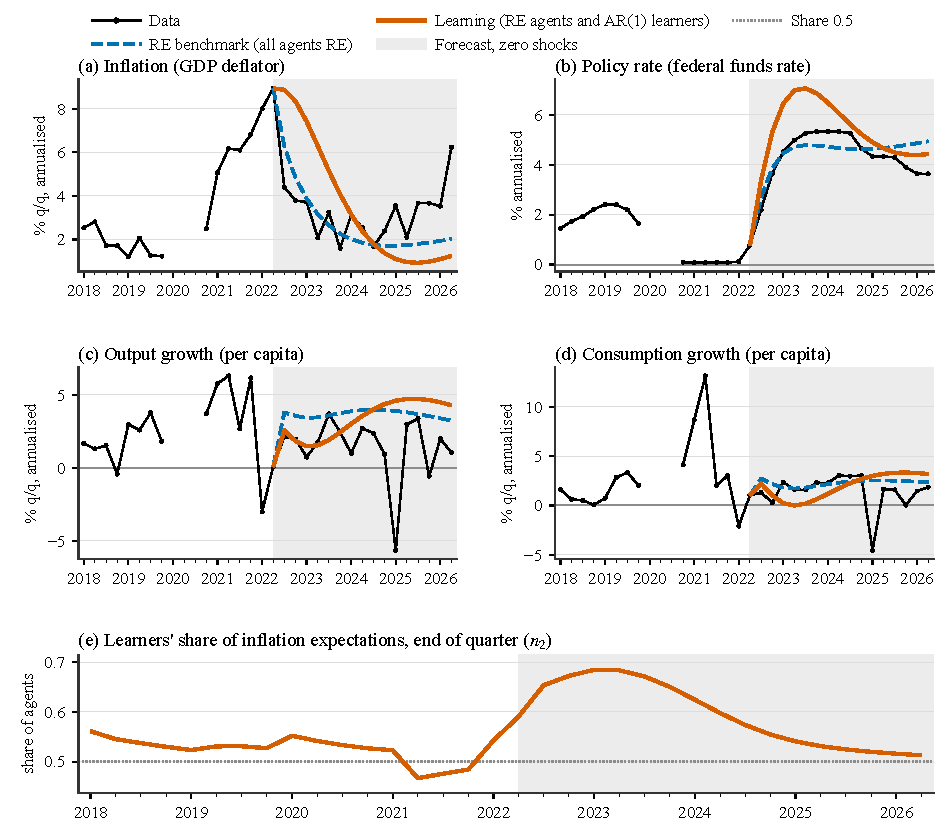
\includegraphics[width=\textwidth]{figures/fig_app1.pdf}
\caption{Application 1: forecast from the 2022Q2 inflation peak with zero future shocks.
Panels (a)--(d): data (black, with a gap in 2020Q1--2020Q3, treated as missing), the RE
benchmark (blue, dashed) and the learning economy with anchored RE agents and AR(1) learners on
inflation expectations (vermillion), in percent, quarter-on-quarter annualised (policy rate:
percent a year). Panel (e): the learners' share at the end of each quarter, $n_2 = 1-n_1$, which
is the share in force in the next quarter. The forecast period is shaded.}
\label{fig:app1}
\end{figure}

{\let\small\relax\setlength{\tabcolsep}{4pt}\begin{table}[tbp]
\centering
\small
\caption{Application 1: forecast from the 2022Q2 peak, average outcomes}
\label{tab:app1}
\begin{tabular}{lrrrrrrrr}
\toprule
& \multicolumn{4}{c}{2022Q3--2023Q2} & \multicolumn{4}{c}{2022Q3--2026Q2} \\
\cmidrule(lr){2-5}\cmidrule(lr){6-9}
Variable & Data & RE & Learning & L $-$ RE & Data & RE & Learning & L $-$ RE \\
\midrule
Inflation & 3.50 & 4.54 & 7.73 & +3.20 & 3.21 & 2.59 & 3.45 & +0.86 \\
Policy rate & 3.84 & 3.93 & 5.53 & +1.59 & 4.41 & 4.53 & 5.42 & +0.88 \\
Output growth & 1.65 & 3.57 & 1.86 & $-$1.70 & 1.44 & 3.69 & 3.39 & $-$0.29 \\
Consumption growth & 1.38 & 2.10 & 0.86 & $-$1.24 & 1.42 & 2.27 & 1.96 & $-$0.31 \\
\bottomrule
\end{tabular}
\par\smallskip
\begin{minipage}{\linewidth}\footnotesize
\textit{Notes:} Averages of the forecast from the 2022Q2 inflation peak with zero future shocks, in \% (inflation: GDP deflator, q/q annualised; output and consumption growth: per capita, q/q annualised; policy rate: federal funds rate, \% a year). L $-$ RE: learning minus RE, pp. RE: every agent rational, RE information $t-1$. Learning: anchored RE agents and AR(1) learners on inflation expectations with switching shares (KOZ gain, $\chi=2$, memory 0.8). Data: the realised values, for comparison. Learners' share at the end of 2022Q2: 0.591; peak in the forecast 0.685 (2023Q1); learners' AR(1) coefficient at the origin 1.061. Source: \texttt{paths\_long.csv}, \texttt{learning\_long.csv}.
\end{minipage}
\end{table}
}

The mechanism is visible in the learning state, which the toolbox records for every quarter of
the history and the forecast (Figure~\ref{fig:history}). Over 1966Q1--2022Q2 the learners'
perceived AR(1) coefficient averages 0.75. It was 0.32 at the end of 2019 and rose to 1.06 by
2022Q2, one of only three quarters in the sample (with 1974Q3 and 2022Q1) in which it reached one.
Learners therefore enter the forecast with an explosive perceived law of motion and extrapolate
the peak; the facility setting of the baseline allows this as long as the model solves, and it
never acts in this run. Their share rose from 0.47 at the end of 2021Q2 to 0.59 at the end of
2022Q2, as their forecasts beat the RE forecasts during the surge. In the zero-shock forecast the
share keeps rising to 0.69 in 2023Q1 and then drifts back towards one half, as both forecast errors
shrink. On the data that followed, the share instead fell to 0.23 in 2022Q4, its lowest value since
1966: realised inflation fell faster than the learners' AR(1) predicted.

\begin{figure}[tbp]
\centering
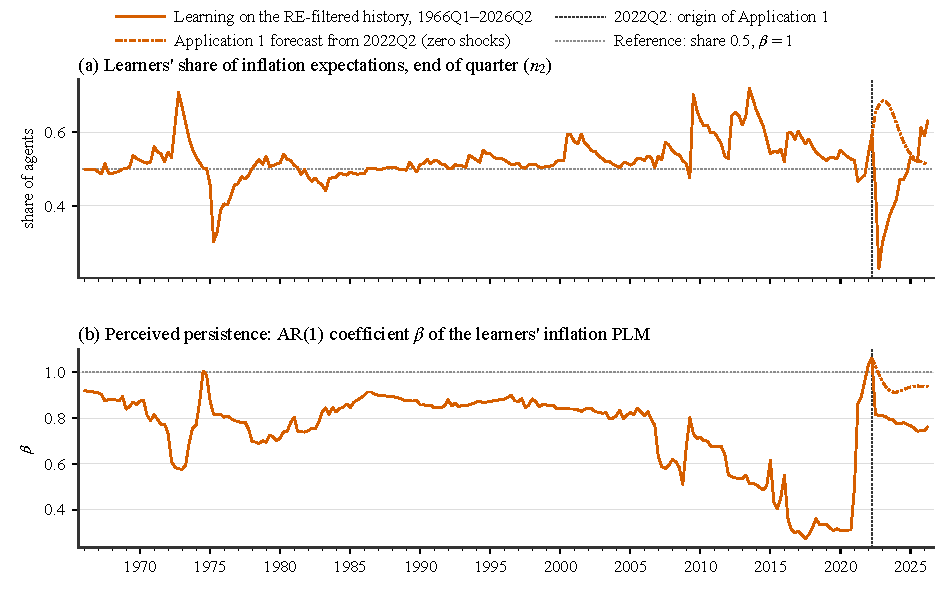
\includegraphics[width=\textwidth]{figures/fig_history.pdf}
\caption{Learning state of Application 1 over 1966Q1--2026Q2. (a) Learners' share of inflation
expectations at the end of each quarter. (b) The AR(1) coefficient $\beta$ of the learners'
inflation PLM. Solid: learning on the RE-filtered history through 2026Q2 (the run equals
Application 1 up to 2022Q2). Dash-dot: the Application 1 forecast from 2022Q2 with zero
shocks. Dotted lines: share 0.5 and $\beta = 1$.}
\label{fig:history}
\end{figure}

The benchmark and the learning economy are two scenario files that differ in one option, the
mode: \code{'rational'} for the benchmark and \code{'switching'} for the learning economy.

\subsection{Application 3: a deviation from the policy rule}\label{sec:app3}

Application~3 holds the policy rate 100 basis points a year below (looser) or above (tighter)
the Taylor rule for four quarters, 2022Q3--2023Q2, using the condition of
Section~\ref{sec:scenarios}: the policy-shock process is held 0.25 percentage points per quarter
off its path in the same scenario without the condition, and the monetary policy shock is
endogenised to deliver it. Figure~\ref{fig:app3} shows the effects as deviations from
Application~1. Under learning the inflation effect comes later and is slightly larger: it peaks at
0.72 percentage points in 2024Q1 for the looser policy, against 0.67 points in 2023Q3 under RE.
Under RE the looser and tighter runs are mirror images (their sum is zero to $10^{-13}$). Under
learning they are not, because the policy deviation moves the learners' share in force: up by as
much as 0.024 with looser policy and down by as much as 0.030 with tighter policy. The asymmetry is
small here, about 2\% of the inflation effect at its largest, but the toolbox measures it directly
by running the two scenarios.

\begin{figure}[tbp]
\centering
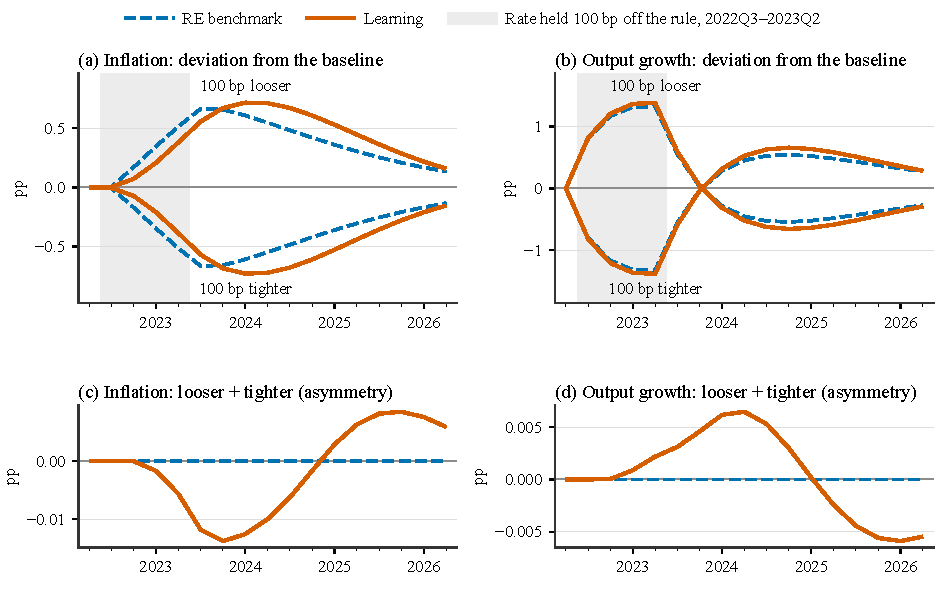
\includegraphics[width=\textwidth]{figures/fig_app3.pdf}
\caption{Application 3: policy rate held 100 basis points a year below or above the Taylor rule
in 2022Q3--2023Q2 (shaded), from the 2022Q2 peak. (a), (b): deviations of inflation and output
growth from Application 1, in percentage points of the annualised rates, under RE (blue, dashed)
and learning (vermillion). (c), (d): the sum of the looser and tighter deviations, which is zero
when the two responses are symmetric.}
\label{fig:app3}
\end{figure}

\subsection{Application 4: Ramsey policy}\label{sec:app4}

Application~4 replaces the Taylor rule by Ramsey policy under commitment from the 2022Q2 origin.
The loss puts weight 1 on annualised inflation, 0.5 on the output gap (output relative to its
flexible-price level) and 0.1 on the annualised policy rate, discounted with the discount factor
of the SW07 Phillips curve. Ramsey policy is not available with lagged RE information, so all runs
of this application give RE agents period-$t$ information, and their rule paths differ from those
of Application~1. The RE Ramsey benchmark uses model-consistent RE agents, so that RE agents
forecast the economy under the Ramsey policy.

\begin{figure}[tbp]
\centering
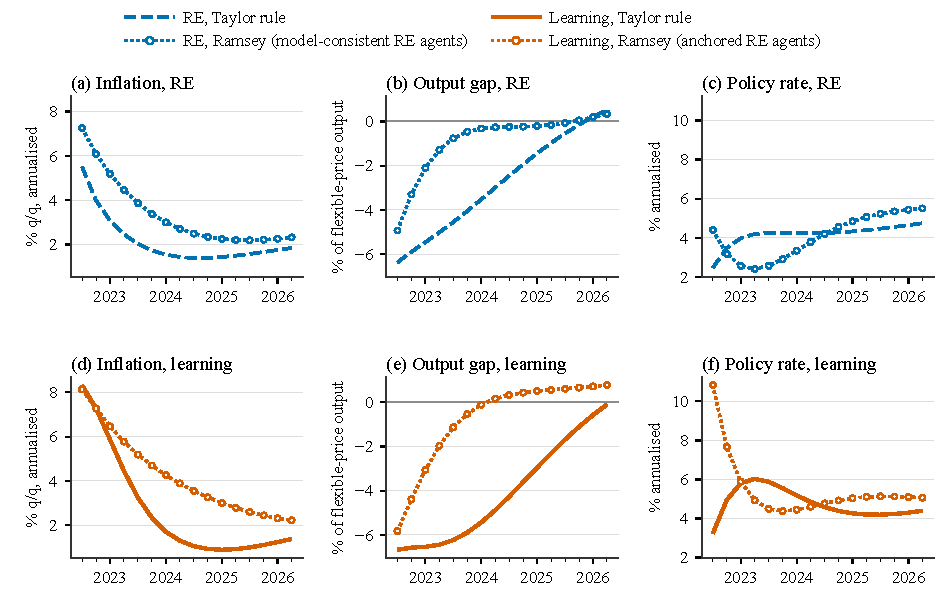
\includegraphics[width=\textwidth]{figures/fig_app4.pdf}
\caption{Application 4: Ramsey policy under commitment against the Taylor rule from the 2022Q2
peak, zero shocks, loss weights 1 (inflation), 0.5 (output gap) and 0.1 (policy rate). Top row: RE,
with model-consistent RE agents under Ramsey policy. Bottom row: learning, with anchored RE agents
who keep the RE forecast under the Taylor rule. Inflation and policy rate in percent annualised;
output gap in percent of flexible-price output.}
\label{fig:app4}
\end{figure}

{\let\small\relax\setlength{\tabcolsep}{4pt}\begin{table}[tbp]
\centering
\small
\caption{Application 4: Ramsey policy against the Taylor rule}
\label{tab:app4}
\begin{tabular}{lrrrrrrrrr}
\toprule
& \multicolumn{3}{c}{Loss weights} & \multicolumn{3}{c}{RE} & \multicolumn{3}{c}{Learning} \\
\cmidrule(lr){2-4}\cmidrule(lr){5-7}\cmidrule(lr){8-10}
Weights & $\lambda_y$ & $\lambda_r$ & $\lambda_{\Delta r}$ & Rule & Ramsey & Ratio & Rule & Ramsey & Ratio \\
\midrule
\multicolumn{10}{l}{\textit{Discounted loss over 80 quarters}} \\
\quad Balanced & 0.5 & 0.1 & 0 & 230.1 & 127.7 & 0.56 & 359.4 & 184.5 & 0.51 \\
\quad Hawk & 0.1 & 0.1 & 0 & 104.9 & 51.5 & 0.49 & 175.4 & 94.6 & 0.54 \\
\quad Dove & 1 & 0.1 & 0 & 386.6 & 196.2 & 0.51 & 589.4 & 234.2 & 0.40 \\
\quad Smooth & 0.5 & 0.1 & 0.5 & 232.2 & 129.6 & 0.56 & 364.6 & 201.0 & 0.55 \\
\addlinespace
\multicolumn{10}{l}{\textit{Discounted loss over 16 quarters}} \\
\quad Balanced & 0.5 & 0.1 & 0 & 146.7 & 68.2 & 0.47 & 270.4 & 106.4 & 0.39 \\
\quad Hawk & 0.1 & 0.1 & 0 & 66.7 & 37.7 & 0.57 & 133.1 & 64.6 & 0.49 \\
\quad Dove & 1 & 0.1 & 0 & 246.7 & 87.9 & 0.36 & 442.0 & 135.9 & 0.31 \\
\quad Smooth & 0.5 & 0.1 & 0.5 & 148.8 & 70.2 & 0.47 & 275.6 & 123.1 & 0.45 \\
\addlinespace
\multicolumn{10}{l}{\textit{Balanced weights: averages 2022Q3--2026Q2}} \\
\quad Inflation (\%) & & & & 2.14 & 3.39 & & 2.69 & 4.24 & \\
\quad Output gap (\%) & & & & $-$2.79 & $-$0.86 & & $-$4.08 & $-$0.77 & \\
\quad Policy rate (\%) & & & & 4.17 & 4.08 & & 4.75 & 5.47 & \\
\bottomrule
\end{tabular}
\par\smallskip
\begin{minipage}{\linewidth}\footnotesize
\textit{Notes:} Taylor rule against Ramsey policy under commitment from the 2022Q2 peak, zero shocks. Loss $= \sum_h \delta^h(\hat\pi_h^2 + \lambda_y x_h^2 + \lambda_r \hat r_h^2 + \lambda_{\Delta r} (\Delta \hat r_h)^2)$, where $\hat\pi = 4\pi$ and $\hat r = 4r$ are annualised deviations of inflation and the policy rate from the steady state, $x = y-y^f$ is the output gap, the weight on inflation is 1 and $\delta = \bar\beta\gamma$ is the discount of the SW07 Phillips curve; the 80-quarter loss continues the forecast with zero shocks. Ratio: Ramsey / rule. RE Ramsey: the model-consistent RE plan (RE agents forecast the economy under the Ramsey policy). Learning Ramsey: the anchored RE agents keep the Taylor-rule RE forecast, so its loss is not a clean gain from optimal policy. All runs use period-$t$ RE information. Anchored RE Ramsey losses over 80 quarters (not RE plans): balanced 125.0, hawk 51.5, dove 162.8, smooth 129.8. Source: \texttt{app4\_losses.csv}, \texttt{app4\_targets\_long.csv}, \texttt{paths\_long.csv}.
\end{minipage}
\end{table}
}

Figure~\ref{fig:app4} and Table~\ref{tab:app4} show the results. In both economies the planner
lets inflation fall more slowly than the rule does and closes the output gap much faster. Under
RE average inflation over the four years is 3.39\% under Ramsey policy against 2.14\% under the
rule, and the average output gap $-0.86\%$ against $-2.79\%$; with learners the figures are
4.24\% against 2.69\%, and $-0.77\%$ against $-4.08\%$. With learners the planner raises the
policy rate to 10.8\% in the first quarter, from 0.77\% at the origin, against 4.4\% under RE.
The discounted loss over 80 quarters falls from 230.1 to 127.7 under RE and from 359.4 to 184.5
with learners, and Ramsey policy roughly halves the loss for each of the four weight sets in
Table~\ref{tab:app4}.

The learning comparison has a caveat. The anchored RE agents of the learning economy forecast
with the RE solution under the Taylor rule, not under the Ramsey policy, so the learning Ramsey
loss is not a clean measure of the gain from optimal policy. The assumption also matters in the
RE economy: with anchored instead of model-consistent agents, the balanced-weight Ramsey loss is
125.0 instead of 127.7 (notes of Table~\ref{tab:app4}), and those anchored runs are not RE
plans. A modeler who wants RE
agents to know the Ramsey policy in the learning economy can set them to model-consistent; which
assumption is appropriate is a modeling choice, not a property of the toolbox.

\subsection{Density forecasts}\label{sec:app5}

Figure~\ref{fig:density} shows density forecasts from the same origin with 500 draws of normal
shocks with the model's standard deviations, under RE and with learners, for two groups of shocks:
the price and wage mark-up shocks (supply), and the risk-premium, government-spending and
investment shocks (demand). The draws are the same in both economies. With mark-up shocks the 90\%
band of inflation is on average 14.6 percentage points wide with learners against 4.8 points under
RE, about three times as wide, and skewed upwards: in 2026Q2 it runs from $-2.0\%$ to $16.6\%$
against $-1.0\%$ to $4.6\%$. Inflation shocks feed the learners' explosive beliefs and raise their
share. The band of output growth is also wider (7.5 against 3.0 points). With demand shocks the
bands are about the same in both economies (1.2 points for inflation and about 10 points for output
growth). The projection facility acted in 23 of the 500 learning draws with mark-up shocks,
reverting beliefs in 46 quarters and keeping the previous shares in 13, and in none of the demand
draws; every draw completed and is used.

\begin{figure}[tbp]
\centering
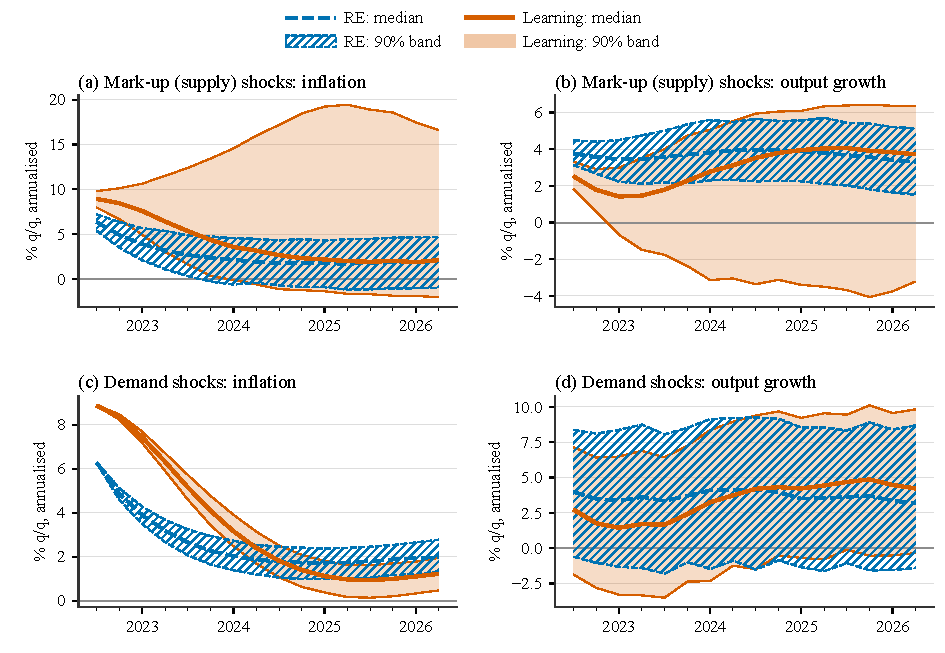
\includegraphics[width=\textwidth]{figures/fig_density.pdf}
\caption{Density forecasts from the 2022Q2 peak: medians and 90\% bands (5th to 95th percentiles)
of 500 stochastic forecasts with normal draws of the model's shock standard deviations (seed 0).
Top: price and wage mark-up shocks. Bottom: risk-premium, government-spending and investment
shocks. RE: dashed median, hatched band. Learning: solid median, filled band. Percent,
quarter-on-quarter annualised.}
\label{fig:density}
\end{figure}

\subsection{Alternative perceived laws of motion}\label{sec:plm}

The last illustration changes only the learners' PLM for inflation. Each variant is a few lines of
options on the baseline: \code{beliefs.plm.default = 'ar2'} for the AR(2); a derived output gap
\code{y - yf} and \code{beliefs.plm.var} over inflation, the output gap and the policy rate for the
three-variable VAR(1); a VAR(1) over the twelve forward-looking variables. In every variant only
inflation expectations are heterogeneous; the other equations of a VAR forecast the regressors.

\begin{figure}[tbp]
\centering
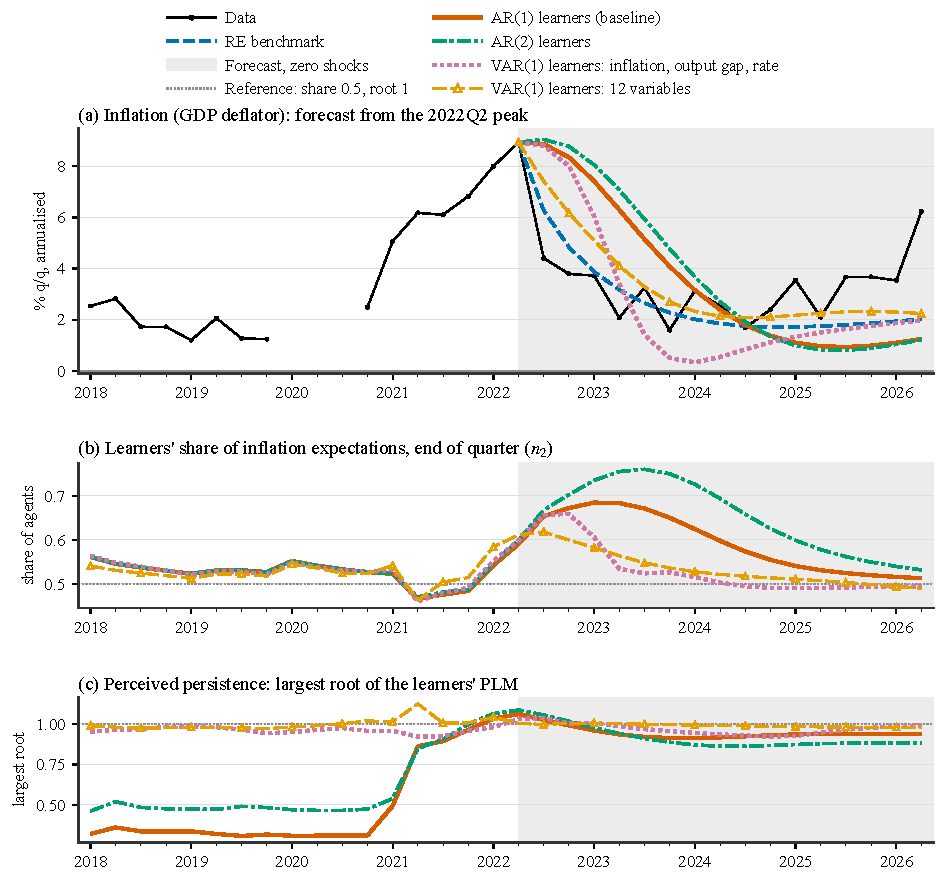
\includegraphics[width=\textwidth]{figures/fig_plm.pdf}
\caption{Application 1 with four PLMs for the inflation learners: AR(1) (baseline), AR(2), a
VAR(1) in inflation, the output gap and the policy rate, and a VAR(1) in the twelve
forward-looking variables. (a) Inflation with the data and the RE benchmark, percent annualised.
(b) Learners' share at the end of each quarter. (c) Largest root of the PLM (for the AR(1), the
coefficient $\beta$). The forecast period is shaded.}
\label{fig:plm}
\end{figure}

{\let\small\relax\setlength{\tabcolsep}{4pt}\begin{table}[tbp]
\centering
\small
\caption{Perceived laws of motion: Application 1 with alternative PLMs}
\label{tab:plm}
\begin{tabular}{lrrrrrrr}
\toprule
& \multicolumn{3}{c}{Average 2022Q3--2026Q2 (\%)} & \multicolumn{2}{c}{Learners' share} & \multicolumn{2}{c}{Largest root} \\
\cmidrule(lr){2-4}\cmidrule(lr){5-6}\cmidrule(lr){7-8}
PLM for inflation & Inflation & Rate & Output gr. & 2022Q2 & Peak & 2022Q2 & Mean 1966--2022 \\
\midrule
RE benchmark & 2.59 & 4.53 & 3.69 & -- & -- & -- & -- \\
\addlinespace
AR(1), baseline & 3.45 & 5.42 & 3.39 & 0.591 & 0.685 & 1.061 & 0.747 \\
AR(1), no constant & 3.25 & 5.18 & 3.46 & 0.611 & 0.651 & 1.031 & 0.883 \\
AR(2) & 3.69 & 5.63 & 3.29 & 0.599 & 0.760 & 1.086 & 0.806 \\
Regression on $\pi$, $x$, $r$ & 2.56 & 4.51 & 3.78 & 0.601 & 0.664 & 1.039 & 0.985 \\
VAR(1) in $\pi$, $x$, $r$ & 2.57 & 4.53 & 3.77 & 0.598 & 0.659 & 1.030 & 0.953 \\
VAR(1) in 12 variables & 3.19 & 5.09 & 3.46 & 0.611 & 0.618 & 1.004 & 0.998 \\
\bottomrule
\end{tabular}
\par\smallskip
\begin{minipage}{\linewidth}\footnotesize
\textit{Notes:} Application 1 (forecast from the 2022Q2 peak, zero shocks) with alternative perceived laws of motion (PLMs) for the inflation learners; everything else as in the baseline. $\pi$: inflation, $x$: output gap, $r$: policy rate; the regression uses their first lags, the 12-variable VAR the 12 forward-looking variables of SW07. Only the inflation expectation uses the PLM; the other equations of the regression and VAR PLMs only forecast the regressors. Learners' share: end-of-quarter share $n_2$ at 2022Q2, and the peak share in force ($n_2$ of the previous quarter) over 2022Q3--2026Q2. Largest root of the PLM block (the AR(1) coefficient for the AR(1) PLMs) at 2022Q2 and its mean over 1966Q1--2022Q2. No projection-facility events in any of these runs. Source: \texttt{paths\_long.csv}, \texttt{learning\_long.csv}.
\end{minipage}
\end{table}
}

Figure~\ref{fig:plm} and Table~\ref{tab:plm} show that the PLM matters as much as the presence of
learners. Average inflation over the four years ranges from 2.56\% (a regression on lagged
inflation, output gap and policy rate) to 3.69\% (AR(2)), a wider spread than the gap between
the baseline learning economy and RE (3.45\% against 2.59\%). Every PLM has a largest root at or above one at the
origin, but they differ in how they got there: averaged over 1966Q1--2022Q2 the largest root is
0.75 for the AR(1), 0.81 for the AR(2), 0.95 for the three-variable VAR(1) and 1.00 for the
twelve-variable VAR(1), whose learners perceive inflation as close to a unit root throughout the
sample. The shares at the origin are close (0.59 to 0.61), but the AR(2) learners gain more
ground in the forecast, to a peak share of 0.76. No variant triggers the projection facility.

\subsection{Other tools run on SW07}\label{sec:other}

The repository runs the remaining tools on the same model; their results are documented on the
website and not reported here. Application~2 replays the RE-smoothed shocks of 2022Q3--2026Q2
through the learning economy. Application~6 builds the history with the inversion and with the
Kalman filter and decomposes the learning paths into shocks with time-varying beliefs. Model variants switch the RE agents to model-consistent,
put all twelve forward-looking variables in the learning set, and replace the KOZ gain by a
constant gain. A real-time evaluation scores ten variants at 138 forecast origins with
Diebold--Mariano tests. Each is a folder of scenario files and one call to the project's runner.

% =====================================================================================
\section{Further expectation rules}\label{sec:rules}
% =====================================================================================

The two-type structure of the previous sections is a special case of a more general one that the
toolbox also contains. Three options extend it. Agent types (\code{expectations.types}) replace
the pair of RE agents and learners by a list of types, each of one of four kinds: the RE type, a
learner with a PLM, a fixed linear forecasting rule, or an RE forecast plus a learned mean of its
own past errors. Shares over $N$ types follow the same logit as before,
\begin{equation}\label{eq:ntypes}
  U_{k,t} = \omega\,U_{k,t-1} - (1-\omega)\,\FE_{k,t}, \qquad
  n_{k,t} = \frac{\exp(\chi U_{k,t})}{\sum_{j=1}^{N}\exp(\chi U_{j,t})},
\end{equation}
with initial or fixed shares set by type (\code{shares.init}, \code{shares.fixed}). Forecast
transforms (\code{expectations.transforms}) change an expectation as it enters the model, for
chosen types, variables or single equations: a multiplier, a diagnostic distortion, or a mix of
the forecast and a lagged value. Fitness is computed on the transformed forecasts. All three are
off by default, and a run that sets none of them takes the two-type code unchanged; a regression
test checks that the two-type results are exactly those obtained before the extensions were added.
The extensions work with the RE-smoother and Kalman histories, the forecast stage, density
forecasts, the forecast evaluation and the decompositions. They are not available with the
inversion history or with Ramsey policy.

Seven rules from the bounded-rationality literature are built with these options and kept as
scenario files, each adding a few lines to the baseline of Application~1 (Table~\ref{tab:rules}).
Their parameter values come from published estimates, mostly made in other models, so they are
starting points rather than calibrations for SW07.

\begin{table}[tbp]
\centering
\setlength{\tabcolsep}{4pt}
\caption{Further expectation rules included in the toolbox}
\label{tab:rules}
\begin{tabular}{>{\raggedright\arraybackslash}p{2.5cm}>{\raggedright\arraybackslash}p{2.5cm}>{\raggedright\arraybackslash}p{4.8cm}>{\raggedright\arraybackslash}p{1.8cm}}
\toprule
Rule & Source & How it is expressed & Value \\
\midrule
Cognitive discounting on the learning set & \citet{gabaix2020}; \citet{meggiorini2021} & multiplier $m^h$ on the inflation expectations of both types ($h=2$ for a forecast made with data up to $t-1$) & $m=0.94$ \\
\addlinespace
Myopia and anchoring & \citet{angeletos2021} & the inflation expectation in the price Phillips curve becomes $\omega_f f + b\,\pi_{t-1}$ & $\omega_f=0.52$, $b=0.434$ \\
\addlinespace
Diagnostic expectations & \citet{bordalo2018}; \citet{lhuillier2024} & RE expectations become $(1+\theta)f_t - \theta f_{t-1}$, with $f_{t-1}$ the same forecast made a quarter earlier; flexible-price block excluded & $\theta=0.44$ \\
\addlinespace
Target believers & \citet{hommes2019} & a third type that forecasts the steady state, switching with RE agents and learners & initial shares $1/3$ \\
\addlinespace
Intercept-only learners & \citet{gati2023}; \citet{carvalho2023} & in place of the AR(1) learners: the RE forecast plus a learned mean of its past errors & baseline gain \\
\addlinespace
Mean-only learners & adaptive expectations & PLM with a constant only, so RLS is exponential smoothing & baseline gain \\
\addlinespace
Experience-based gain & \citet{malmendier2016}; \citet{nagel2022} & AR(1) learners with a constant gain in place of the KOZ gain; no cohorts & 0.018 a quarter \\
\bottomrule
\end{tabular}
\par\smallskip
\begin{minipage}{\linewidth}\footnotesize
\textit{Notes:} Each rule is a scenario file that adds its lines to the Application 1 baseline,
in which inflation expectations are heterogeneous. Values: $m$ from \citet{meggiorini2021},
estimated with learners on US data for 1960--2007; $\omega_f$ and the backward weight from
\citet{angeletos2021}; $\theta$ from \citet{lhuillier2024}; the gain from \citet{malmendier2016}
as used by \citet{nagel2022}. The initial shares of the target believers are a choice, not an
estimate.
\end{minipage}
\end{table}

Cognitive discounting \citep{gabaix2020} shrinks expectations towards the steady state by a factor
$m<1$ per period of horizon; following \citet{meggiorini2021}, who estimate it together with
learning, the multiplier applies to the expectations of the learning set, of RE agents and
learners alike. Myopia and anchoring \citep{angeletos2021} replace the forward-looking term of the
price Phillips curve by a damped expectation plus a backward-looking term, with weights from their
calibration; SW07 keeps its own price indexation, so the backward weight comes on top of it.
Diagnostic expectations \citep{bordalo2018,lhuillier2024} overweight the news in the latest
forecast revision; the transform applies to the RE agents and to the model-consistent
expectations, while the learners are left as they are. Target believers \citep{hommes2019} add a
type whose forecast is the inflation target (here the steady state), so their share can be read as
credibility. Intercept-only learners, in the spirit of \citet{gati2023} and \citet{carvalho2023},
use the RE slopes but learn the mean of their own forecast errors, so their expectations can drift
away from the RE mean; the smooth anchoring function of \citet{gati2023} is not included.
Mean-only learners forecast the learned mean, which is adaptive expectations. The experience-based
gain uses the constant gain that \citet{nagel2022} derive from the cohort learning of
\citet{malmendier2016}, without the cohorts.

The rules run through Application~1 and through impulse responses and in-sample fit with the Kalman
history in the repository. They are listed here so that readers know they are available; this
paper does not report their results.

% =====================================================================================
\section{Extending the toolbox, and its limits}\label{sec:extend}
% =====================================================================================

\subsection{Extension points}\label{sec:extpoints}

The toolbox is built so that the common extensions do not touch the engine.

\begin{itemize}
\item \emph{A new model} is a new package (Section~\ref{sec:package}). The generator, the collapse
      test and the RE filter handle the rest, and a load call lists the forward-looking variables
      that can learn. The documentation website walks through the steps with one of the template
      packages.
\item \emph{A new gain rule} is a MATLAB function with four calls: the series it records, its
      initial state, the gains of the current quarter's updates and the state update at the end of
      the quarter. Its state is stored in the learning state, so every stage carries it without
      further code. The KOZ gain is implemented this way.
\item \emph{A new switching rule} is a function with the interface of the discrete-choice rule:
      squared errors and previous fitness in, shares and new fitness out, vectorised over share
      groups.
\item \emph{A new PLM} is, in most cases, an option: any linear regression on lagged transition
      variables, derived variables or VAR blocks can be written with \code{beliefs.plm.by_var},
      \code{.derived} and \code{.var}.
\item \emph{A new expectation rule} can often be expressed with the agent types and transforms
      of Section~\ref{sec:rules}: a fixed rule is a linear expression in lagged variables, and a
      transform changes the expectation of chosen types in chosen equations.
\item \emph{A new application} is a scenario file that inherits from an existing one. Option
      names are checked, so a misspelt field fails at once, and every result stores its options,
      so saved runs can be reproduced.
\end{itemize}

\subsection{Limitations}\label{sec:limits}

\begin{itemize}
\item The toolbox has been tested on linear models with linear solutions only. A nonlinear model
      has a code path (a steady-state call before each solve) but no test; the anchored RE variant
      and the backward simulator are linear only, and log variables are not read by the fast
      one-period step or the Kalman history.
\item Shocks and conditions are unanticipated. Anticipated paths, such as announced policy, are
      not implemented.
\item Agents and the Ramsey planner treat current beliefs and shares as permanent (anticipated
      utility); nobody anticipates future learning.
\item Ramsey policy is not available with lagged RE information. Discretion can be indeterminate
      in IRIS at some parameter points, and anchored RE agents keep the reduced form under the rule.
\item With zero future shocks the shares drift towards one half, since forecast errors vanish
      for both types.
\item The forecast evaluation uses the current data vintage and fixed parameters; only the
      history and the starting state are real time.
\item The toolbox does not estimate parameters. Learning parameters such as the gain, $\chi$ and
      $\omega$ are inputs, and so are the model's structural parameters.
\item The tested versions are IRIS release 20230622 and MATLAB R2025a. The optimal-policy parser
      of that IRIS release fails on MATLAB R2025a, and the repository ships a corrected copy of the
      one IRIS file involved.
\end{itemize}

The cost of the quarter-by-quarter approach is computing time, since the model is re-solved
whenever beliefs or shares change. On the machine used for this paper, a single SW07 scenario takes
between a few seconds and half a minute once the generated files and filter caches exist, a
learning density forecast
about one second per draw, and the evaluation of ten variants at 138 origins a little over an hour
of computing time, which the runner splits across parallel MATLAB sessions.
% TODO(author): add the machine (CPU, memory) and confirm the timings; they come from the run
% log of 2026-10-18 to 2026-10-21 in README_PIPELINE.md.

% =====================================================================================
\section{Conclusion}\label{sec:concl}
% =====================================================================================

hetlearn turns an IRIS model with forward-looking terms into a model with heterogeneous
expectations, adaptive learning and switching, without changes to the model file. Its options cover
the choices on which the learning literature differs (information timing, the type of RE agent, the
PLM, initial beliefs, gains, switching and stabilisation) and the analyses a forecaster needs
(unconditional and conditional forecasts, Ramsey policy, densities, decompositions and real-time
evaluation), with the RE benchmark always one option away. The SW07 illustrations show what this
gives in practice: the same forecast from the 2022 inflation peak can be read under RE, under
learning, under a policy deviation, under optimal policy, as a density and with different PLMs,
and in each case the learning state that drives the result is recorded quarter by quarter.

The toolbox does not settle which expectation assumption is right; it makes the comparison cheap.
Natural next steps are tests on further models, including nonlinear ones, anticipated policy
paths, and the estimation of learning parameters, which this paper leaves out. The documentation
website and the technical appendix in the repository describe every option in more detail than
this paper can.

\backmatter

\bmhead{Acknowledgements}

% TODO(author): acknowledgements, or delete this heading.
[Acknowledgements to be added.]

\section*{Declarations}

\begin{itemize}
\item \textbf{Funding.} [To be completed by the author.]
% TODO(author): funding statement, or "No funding was received for this work."
\item \textbf{Competing interests.} [To be completed by the author; for example: the author has
      no competing interests to declare.]
\item \textbf{Data availability.} The illustrations use US macroeconomic series from FRED, Federal
      Reserve Bank of St.\ Louis (vintage of 29 September 2026), transformed as in
      \citet{smets2007}. The database and the scripts that build it are in the code repository.
\item \textbf{Code availability.} The toolbox, the SW07 model package, the scenario files and the
      scripts that produce every figure and table of this paper are in the repository
      \url{https://github.com/tolgaozden/iris_toolbox_learning}. Documentation:
      \url{https://tolgaozden.github.io/iris_toolbox_learning/}.
% TODO(author): the repository is private and the site is not yet deployed. Make the repository
% public (or archive a release on Zenodo with a DOI) before submission, and update this statement.
\item \textbf{Disclaimer.} [Disclaimer to be added by the author: the views expressed are those of
      the author and do not necessarily reflect those of the author's institution.]
\end{itemize}

\begin{appendices}

\section{Reproducing the figures and tables}\label{app:repro}

Every figure and table of Section~\ref{sec:sw07} is drawn from saved runs of scenario files in
\code{scenarios/sw07/}. Table~\ref{tab:repro} lists them with the group of the project's runner
that produces them. From the project root, in MATLAB with IRIS 20230622 installed:
\begin{lstlisting}
setup_paths                      % IRIS, the toolbox and the scenarios
run_applications('all')          % every group, the evaluation included
run('results/summary_v3/build_summary_v3.m')   % summary CSV files
\end{lstlisting}
and then, in Python, \code{python paper/figures/make_figures.py}, which reads only the summary CSV
files and writes the figures, the tables and a file of the numbers quoted in the text. To rerun
the scenarios of one figure only, pass its group from Table~\ref{tab:repro} to
\code{run_applications}.

\begin{table}[h]
\centering
\setlength{\tabcolsep}{4pt}
\caption{Scenario files behind the figures and tables}
\label{tab:repro}
\begin{tabular}{>{\raggedright\arraybackslash}p{2.8cm}>{\raggedright\arraybackslash}p{7.2cm}>{\raggedright\arraybackslash}p{1.6cm}}
\toprule
Output & Scenarios & Group \\
\midrule
Fig.~\ref{fig:app1}, Table~\ref{tab:app1} & \code{a1_re}, \code{a1_learn} & \code{app1} \\
Fig.~\ref{fig:history} & \code{a6_smooth_learn} (\code{a1_learn} with the origin moved to 2026Q2), \code{a1_learn} & \code{app6} \\
Fig.~\ref{fig:app3} & \code{a3_loose_re}, \code{a3_tight_re}, \code{a3_loose_learn}, \code{a3_tight_learn} & \code{app3} \\
Fig.~\ref{fig:app4}, Table~\ref{tab:app4} & \code{a4_rule_re}, \code{a4_rule_learn}, and \code{a4_ramsey_<weights>_re_mc}, \code{_learn}, \code{_re} for four weight sets & \code{app4} \\
Fig.~\ref{fig:density} & \code{a5_markup_re}, \code{a5_markup_learn}, \code{a5_demand_re}, \code{a5_demand_learn} & \code{app5} \\
Fig.~\ref{fig:plm}, Table~\ref{tab:plm} & \code{v2_ar2}, \code{v2_ar1nc}, \code{v2_reg}, \code{v2_var3}, \code{v2_var12} with \code{a1_learn}, \code{a1_re} & \code{var2} \\
\bottomrule
\end{tabular}
\end{table}

\end{appendices}

\bibliography{references}

\end{document}
